\documentclass[tikz]{standalone}
\usepackage{amsmath}
\usepackage{amssymb}
\usepackage{amsfonts}
\usepackage{tikz}

\thispagestyle{empty}
\begin{document}

	
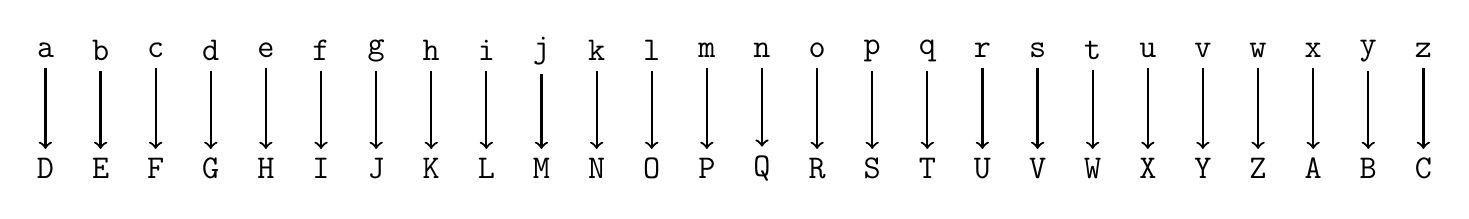
\begin{tikzpicture}[every node/.style={font=\ttfamily\large}, x=0.7cm, y=1.5cm]

% Set the shift amount
\def\shift{3}

% Plaintext row (lowercase)
\foreach \i in {0,...,25} {
	\node (p\i) at (\i, 1) {\char\numexpr`a+\i\relax};
}

% Ciphertext row (uppercase, shifted)
\foreach \i in {0,...,25} {
	\pgfmathsetmacro{\j}{int(mod(\i+\shift,26))}
	\node (c\i) at (\i, 0) {\char\numexpr`A+\j\relax};
}

% Arrows from plaintext to ciphertext
\foreach \i in {0,...,25} {
	\draw[->, thick] (p\i) -- (c\i);
}

\end{tikzpicture}

\end{document}
